\documentclass[12pt,a4paper]{article}
\usepackage[latin1]{inputenc}
\usepackage{amsmath}
\usepackage{amsfonts}
\usepackage{amssymb}
\usepackage{graphicx}
\usepackage{float}
\usepackage{gensymb}
\usepackage{hyperref}
\usepackage{cite}
\usepackage[margin=0.5in]{geometry}
\usepackage[justification=centering, font={small,it}]{caption}
\author{Dicson Wijaya (1002289), Wenkie Lau (1002219), \\ Mok Jun Neng (1002219), Charlotte Phang (1002277), \\ Martin Tan (1002173)}
\title{Systems World 2D Question 3\\ F06 Team 06}

\begin{document}
	
	\maketitle
	
	\section{Part (a)}
	Our objective here is not only to maximise the number of zero coefficients $k_i$'s, but also to have an appropriate minimal chi-square value of the corresponding order controller. In other words, we are required to bring about a balance between these two objectives and present the optimised trade-off in the equation. \\
	
	In order to minimise the number of non-zero coefficients $k_i$'s, we introduce a binary switch $x_i$. \\
	
	Modifying the objective function in question 2, we have: $$Min \ \sum_{n=0}^{9} \bigg( \sum_{i=0}^{9} \frac{(k_i x_i e(n-i) - v(n))^2}{v(n)} \bigg) + \sum_{i=0}^{9} x_i$$ \\
	
	Constraints: $$x_{1,2,3...n} \ \epsilon \ \{ 0,1 \}$$
	
	Decision Variables: $$x_{1,2,3...n} \ , \ k_{1,2,3...n}$$
	
	Parameters: $$e_{1,2,3...9} \ , \ v_{1,2,3...9}$$
	
	\section{Part (b)}
	From question 2, a chi-square distribution with 9 degrees of freedom for a lower one-sided test at significance level $\alpha = 0.001$ has a critical value of 1.152. Therefore, a constraint we set is to have our objective function to be less than or equal to the critical value 1.152. This constraint sets the ceiling or upper bound for the objective function.
	\begin{figure}[H]
		\begin{center}
			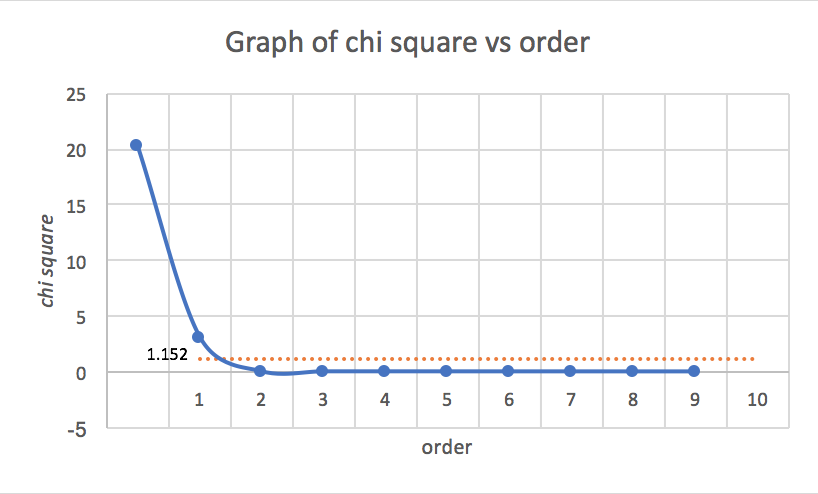
\includegraphics[width=0.75\textwidth]{chi.png}
			\caption{Graph of chi-square values vs order controller}
			\label{fig:chi}
		\end{center}
	\end{figure}
	We multiplied the tabled chi-square values from our answer to question 2 with the binary switch $x_i$'s. This gives us a 10x1 table of chi-square values from each order controller multiplied by the binary switch. Since we can only display the one value that corresponds to the smallest order controller, we set another constraint: sum of binary $x_i = 1$. Hence, only one chi-square value out of the ten data points, corresponding to the smallest order controller, will appear to be non-zero. Since Excel Solver requires the objective function to be a formula, we simply set it as the sum of chi-square vaues with the binary switch on.
	\begin{figure}[H]
		\begin{center}
			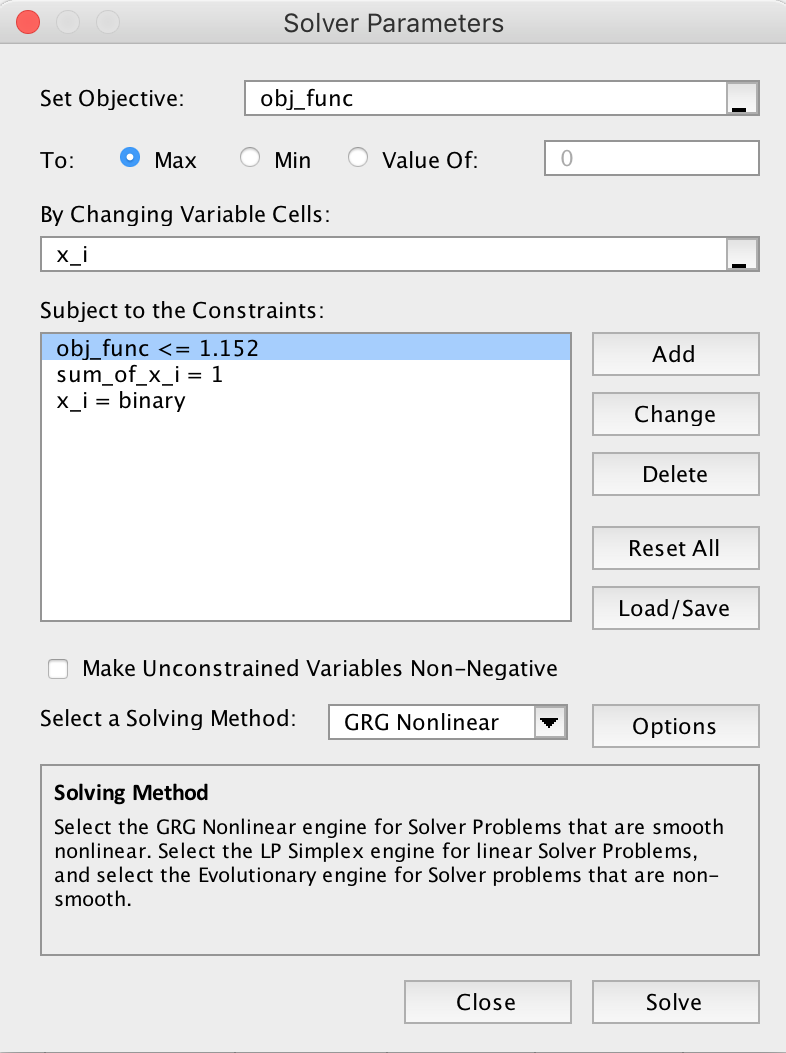
\includegraphics[width=0.45\textwidth]{constraints.png}
			\caption{Constraints to find the objective function in Excel Solver}
			\label{fig:constraints}
		\end{center}
	\end{figure}
    \begin{figure}[H]
    	\begin{center}
    		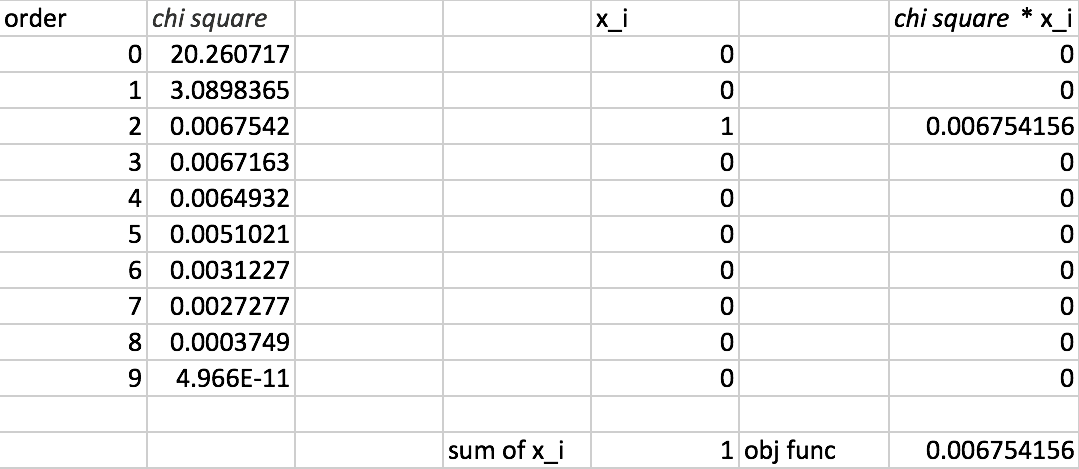
\includegraphics[width=0.75\textwidth]{xcel.png}
    		\caption{Screenshot of the workings in Excel}
    		\label{fig:xcel}
    	\end{center}
    \end{figure}
    The chi-square distribution of calculated v(n) is a convex function. Hence, the smallest order controller is one with a chi-square value just under the ceiling, by the first constraint. Therefore, maximising the objective function gives us the corresponding chi-square value of the smallest order controller: $2^{nd}$ order.
	
\end{document}